% Publication figure generated from the actual h0 reference and
% independently propagated 2h0 local-tip-resolution runs.
% MATLAB source:
%   verification/crack_path/plot_tip2h0_vs_reference_publication.m
%
% Generated vector panels:
%   trajectory.pdf
%   vertical_deviation.pdf
%   direction_deviation.pdf
%   mode_mixity.pdf

\begin{figure}[tbp]
  \centering

  \begin{subfigure}[t]{0.94\linewidth}
    \centering
    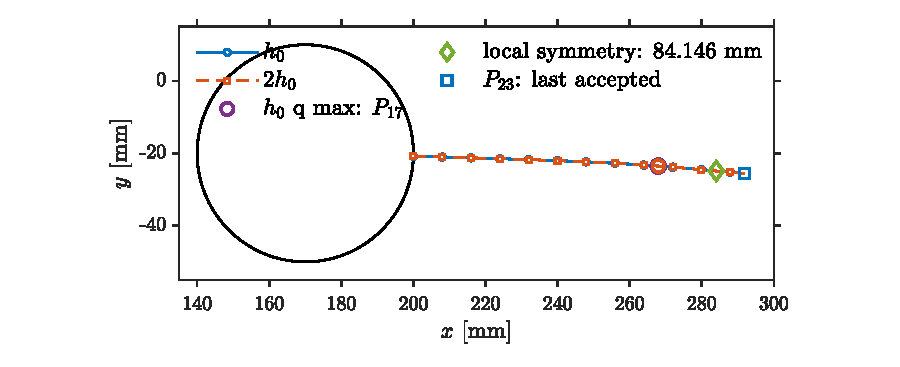
\includegraphics[width=\linewidth]{figures/tip_resolution_sensitivity/trajectory.pdf}
    \caption{Independently propagated trajectories for the production
    tip resolution $h_0$ and the coarser resolution $2h_0$. The two paths
    are visually indistinguishable at the scale of the specimen.}
    \label{fig:tipres-trajectory}
  \end{subfigure}

  \medskip

  \begin{subfigure}[t]{0.315\linewidth}
    \centering
    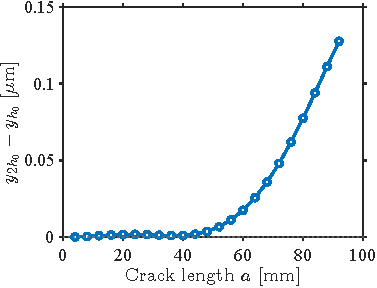
\includegraphics[width=\linewidth]{figures/tip_resolution_sensitivity/vertical_deviation.pdf}
    \caption{Accumulated vertical tip-coordinate difference,
    $y_{2h_0}-y_{h_0}$.}
    \label{fig:tipres-dy}
  \end{subfigure}
  \hfill
  \begin{subfigure}[t]{0.315\linewidth}
    \centering
    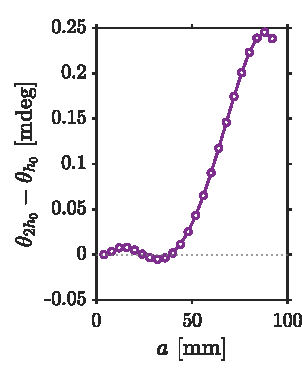
\includegraphics[width=\linewidth]{figures/tip_resolution_sensitivity/direction_deviation.pdf}
    \caption{Difference in the absolute crack direction in the frozen initiation frame,
    $\theta_{2h_0}-\theta_{h_0}$.}
    \label{fig:tipres-dtheta}
  \end{subfigure}
  \hfill
  \begin{subfigure}[t]{0.315\linewidth}
    \centering
    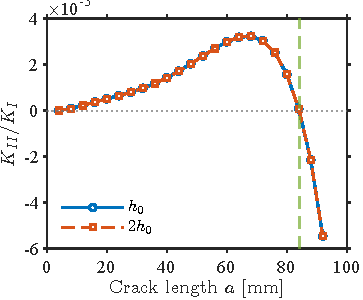
\includegraphics[width=\linewidth]{figures/tip_resolution_sensitivity/mode_mixity.pdf}
    \caption{Mode-mixity ratio $K_{II}/K_I$ along the two independently
    propagated trajectories.}
    \label{fig:tipres-q}
  \end{subfigure}

  \caption{Sensitivity of the incremental LEFM trajectory to the local
  structured tip resolution. The $2h_0$ calculation retains the reference
  exterior mesh law and interaction-domain radii but doubles the production
  tip size from $h_0=0.0270123$ mm to $0.0540247$ mm. The comparison is
  based on two independently propagated trajectories: the $2h_0$ calculation
  recomputes the $P_1$ SIFs and every subsequent MTS update rather than
  reusing reference vertices.}
  \label{fig:tip-resolution-sensitivity}
\end{figure}
